\documentclass{standalone}
\usepackage[utf8]{inputenc}
\usepackage{amsmath}
\usepackage{amsfonts}
\usepackage{amssymb}
\usepackage{tikz}
\usetikzlibrary{calc}

% GanttHeader setups some parameters for the rest of the diagram
% #1 Width of the diagram
% #2 Width of the space reserved for task numbers
% #3 Width of the space reserved for task names
% #4 Number of months in the diagram
% In addition to these parameters, the layout of the diagram is influenced
% by keys defined below, such as y, which changes the vertical scale
\def\GanttHeader#1#2#3#4{%
 \pgfmathparse{(#1-#2-#3)/(#4)}
 \tikzset{y=7mm, task number/.style={left, font=\bfseries},
     task description/.style={text width=#3,  right, draw=none,
           font=\sffamily, xshift=#2,
           minimum height=2em},
     gantt bar/.style={draw=black, fill=blue!30},
     help lines/.style={draw=black!30, dashed},
     x=\pgfmathresult pt
     }
  \def\totalmonths{#4}
  \node (Header) [task description] at (0,0) {\textbf{\large }};
  \begin{scope}[shift=($(Header.south east)$)]
    \foreach \x in {1,...,#4}
      \node[above,rotate=90] at (\x,1) {\tiny\x};
 \end{scope}
}

% This macro adds a task to the diagram
% #1 Number of the task
% #2 Task's name
% #3 Starting date of the task (month's number, can be non-integer)
% #4 Task's duration in months (can be non-integer)
\def\Task#1#2#3#4{%
%\node[task number] at ($(Header.west) + (0, -#1)$) {#1};
\node[task description] at (0,-#1) {#2};
\begin{scope}[shift=($(Header.south east)$)]
  \draw (0,-#1) rectangle +(\totalmonths, 1);
  \foreach \x in {1,...,\totalmonths}
    \draw[help lines] (\x,-#1) -- +(0,1);
  \filldraw[gantt bar] ($(#3, -#1+0.2)$) rectangle +(#4,0.6);
\end{scope}
}

\begin{document}

\begin{tabular}{lr}
Scheduler: & RR-2 scheduler
\\
Input: & input/testdata3.txt
\\
Total Process Count: & 17
\\
Total Waiting Time: & 2094
\\
Average Waiting Time: & 123.17647
\\
Total Turnaround Time: & 2298
\\
Average Turnaround Time: & 135.17647
\\
Total Context Switch Count: & 106
\\
\end{tabular}
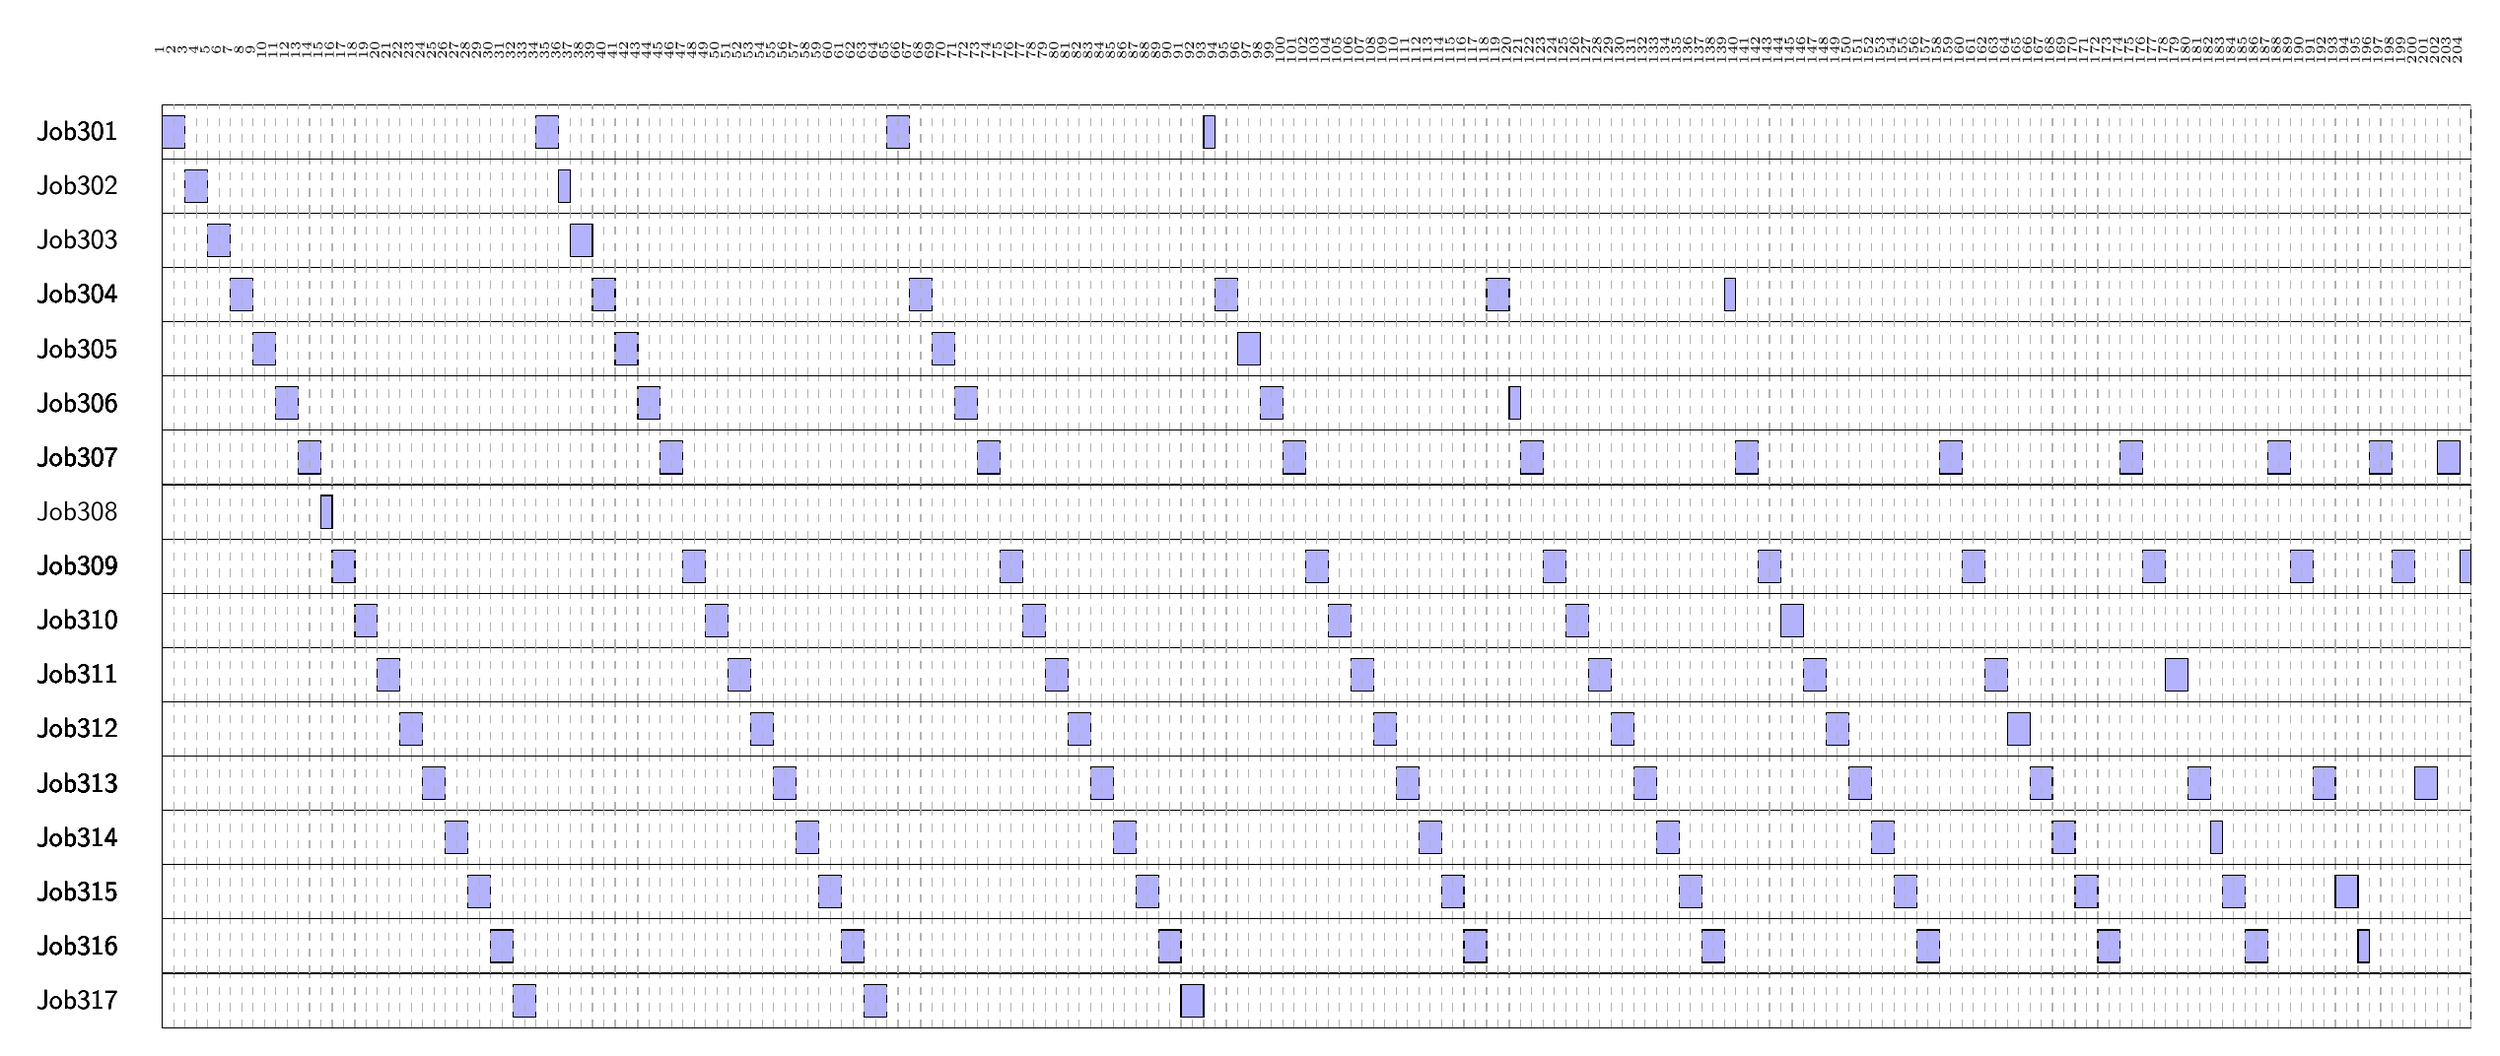
\begin{tikzpicture}
\GanttHeader{32cm}{5ex}{1.5cm}{204}
\Task{1}{Job301}{0}{2}
\Task{2}{Job302}{2}{2}
\Task{3}{Job303}{4}{2}
\Task{4}{Job304}{6}{2}
\Task{5}{Job305}{8}{2}
\Task{6}{Job306}{10}{2}
\Task{7}{Job307}{12}{2}
\Task{8}{Job308}{14}{1}
\Task{9}{Job309}{15}{2}
\Task{10}{Job310}{17}{2}
\Task{11}{Job311}{19}{2}
\Task{12}{Job312}{21}{2}
\Task{13}{Job313}{23}{2}
\Task{14}{Job314}{25}{2}
\Task{15}{Job315}{27}{2}
\Task{16}{Job316}{29}{2}
\Task{17}{Job317}{31}{2}
\Task{1}{Job301}{33}{2}
\Task{2}{Job302}{35}{1}
\Task{3}{Job303}{36}{2}
\Task{4}{Job304}{38}{2}
\Task{5}{Job305}{40}{2}
\Task{6}{Job306}{42}{2}
\Task{7}{Job307}{44}{2}
\Task{9}{Job309}{46}{2}
\Task{10}{Job310}{48}{2}
\Task{11}{Job311}{50}{2}
\Task{12}{Job312}{52}{2}
\Task{13}{Job313}{54}{2}
\Task{14}{Job314}{56}{2}
\Task{15}{Job315}{58}{2}
\Task{16}{Job316}{60}{2}
\Task{17}{Job317}{62}{2}
\Task{1}{Job301}{64}{2}
\Task{4}{Job304}{66}{2}
\Task{5}{Job305}{68}{2}
\Task{6}{Job306}{70}{2}
\Task{7}{Job307}{72}{2}
\Task{9}{Job309}{74}{2}
\Task{10}{Job310}{76}{2}
\Task{11}{Job311}{78}{2}
\Task{12}{Job312}{80}{2}
\Task{13}{Job313}{82}{2}
\Task{14}{Job314}{84}{2}
\Task{15}{Job315}{86}{2}
\Task{16}{Job316}{88}{2}
\Task{17}{Job317}{90}{2}
\Task{1}{Job301}{92}{1}
\Task{4}{Job304}{93}{2}
\Task{5}{Job305}{95}{2}
\Task{6}{Job306}{97}{2}
\Task{7}{Job307}{99}{2}
\Task{9}{Job309}{101}{2}
\Task{10}{Job310}{103}{2}
\Task{11}{Job311}{105}{2}
\Task{12}{Job312}{107}{2}
\Task{13}{Job313}{109}{2}
\Task{14}{Job314}{111}{2}
\Task{15}{Job315}{113}{2}
\Task{16}{Job316}{115}{2}
\Task{4}{Job304}{117}{2}
\Task{6}{Job306}{119}{1}
\Task{7}{Job307}{120}{2}
\Task{9}{Job309}{122}{2}
\Task{10}{Job310}{124}{2}
\Task{11}{Job311}{126}{2}
\Task{12}{Job312}{128}{2}
\Task{13}{Job313}{130}{2}
\Task{14}{Job314}{132}{2}
\Task{15}{Job315}{134}{2}
\Task{16}{Job316}{136}{2}
\Task{4}{Job304}{138}{1}
\Task{7}{Job307}{139}{2}
\Task{9}{Job309}{141}{2}
\Task{10}{Job310}{143}{2}
\Task{11}{Job311}{145}{2}
\Task{12}{Job312}{147}{2}
\Task{13}{Job313}{149}{2}
\Task{14}{Job314}{151}{2}
\Task{15}{Job315}{153}{2}
\Task{16}{Job316}{155}{2}
\Task{7}{Job307}{157}{2}
\Task{9}{Job309}{159}{2}
\Task{11}{Job311}{161}{2}
\Task{12}{Job312}{163}{2}
\Task{13}{Job313}{165}{2}
\Task{14}{Job314}{167}{2}
\Task{15}{Job315}{169}{2}
\Task{16}{Job316}{171}{2}
\Task{7}{Job307}{173}{2}
\Task{9}{Job309}{175}{2}
\Task{11}{Job311}{177}{2}
\Task{13}{Job313}{179}{2}
\Task{14}{Job314}{181}{1}
\Task{15}{Job315}{182}{2}
\Task{16}{Job316}{184}{2}
\Task{7}{Job307}{186}{2}
\Task{9}{Job309}{188}{2}
\Task{13}{Job313}{190}{2}
\Task{15}{Job315}{192}{2}
\Task{16}{Job316}{194}{1}
\Task{7}{Job307}{195}{2}
\Task{9}{Job309}{197}{2}
\Task{13}{Job313}{199}{2}
\Task{7}{Job307}{201}{2}
\Task{9}{Job309}{203}{1}
\end{tikzpicture}
\end{document}
